\section{Spectral Theory} 

  \begin{definition}[Eigenvalue]
    Let $A: V \longrightarrow V$ be a linear transformation over $\mathbb{F}$. If there exists a vector $v \in V$ such that
		\begin{equation}
    	A v = \lambda v, \qquad \lambda \in \mathbb{F}
		\end{equation}
    then $\lambda$ is called an \textbf{eigenvalue} of $A$, and $v$ is an \textbf{eigenvector} of $A$. 
  \end{definition}

  For a given eigenvalue $\lambda$ and its corresponding eigenvector $v$, it is clear that by linearity, every vector in $\Span v$ is an eigenvector, too. 

	\begin{figure}[H]
		\centering 
		\caption{Given a linear transformation $A: V \longrightarrow V$, we can visualize a certain basis of $V$ such that all the linear transformation $A$ does on that basis is merely extend or contract the basis vectors. } 
		\label{fig:eigenvectors}
	\end{figure}

	\begin{definition}[Characteristic Polynomial]
		Let $V$ be a vector space. The \textbf{characteristic polynomial} of linear map $A: V \to V$---denoted $p_A (t)$---is defined
		\begin{equation}
    	p_A (t) \coloneqq \det{(A - t I)}
		\end{equation}
  \end{definition}

	From here, we will assume that our field is over $\mathbb{C}$. We use the fact that the field is over $\mathbb{C}$ because it allows us to claim that the characteristic polynomial in $\mathbb{C}[t]$ can be factored into linear components, by the fundamental theorem of algebra. 

	\begin{lemma}[Invariance of Characteristic Polynomial]
		If two matrices $A, B \in \mathbb{R}^{n \times n}$ are similar, then they have the same characteristic polynomial.
	\end{lemma}
	\begin{proof}
		If $A \sim B$, then $B = S A S^{-1}$, and so 
		\begin{align}
			p_B (t) & = \det(B - tI) \\ 
							&= \det(S A S^{-1} - t SS^{-1}) \\ 
							& = \det(S (A - tI) S^{-1}) \\ 
							& = \det(S) \det(A - tI) \det(S^{-1}) \\ 
							& = \det(A - tI) = p_A (t)
		\end{align}
	\end{proof}

  The motivation for defining such a polynomial is that it allows us to compute the eigenvalues of $A$. 

	\begin{theorem}[Roots of Characteristic Polynomial is the Specturm]
    The solutions of the characteristic equation of $A$ (i.e. the roots of $p_A (t)$) is precisely the spectrum of $A$. 
  \end{theorem}
  \begin{proof} 
    Bidirectional. 
    \begin{enumerate}
      \item $(\rightarrow)$ Let there be a $t = \lambda$ such that $p_A (\lambda) = 0 \iff \det{(A - \lambda I)} = 0$ which is equivalent to saying that ker$(A - \lambda I)$ is nontrivial. There must exist a $v \in $ ker$(A - \lambda I)$, meaning that $(A - \lambda I) v = 0 \iff A v = \lambda v$. By definition, $\lambda$ is an eigenvalue of $A$. 
      \item $(\leftarrow)$ This reasoning can be extended in the opposite direction. 
    \end{enumerate}
  \end{proof}

	Therefore, to find the eigenvalues and eigenvectors, we do the following. First, we solve all zeros of the characteristic polynomial $p_A (t)$. Then, for each zero $\lambda$, we find the corresponding vectors than span $\ker(A - \lambda I)$. 

	\begin{example}[Distinct Eigenvalues]
	  Let 
		\begin{equation}
			A = \begin{pmatrix} 3 & 1 \\ 1 & 2 \end{pmatrix}
		\end{equation}
		Then 
		\begin{equation}
			\det(A - \lambda I) = \det \begin{pmatrix} 3 - \lambda & 1 \\ 1 & 2 - \lambda \end{pmatrix} = (3 - \lambda)(2 - \lambda) - 1 = \lambda^2 - 5 \lambda + 5
		\end{equation}
		So, using the quadratic formula, the eigenvalues of $A$ are 
		\begin{equation}
			\lambda = \frac{5 \pm \sqrt{5}}{2}
		\end{equation}
	\end{example}

	\begin{example}[Same Eigenvalues]
	  Let 
		\begin{equation}
			A = \begin{pmatrix} 2 & 0 & 0 \\ 0 & 2 & 3 \\ 0 & 0 & 5 \end{pmatrix}
		\end{equation}
		Then, 
		\begin{equation}
			\det(A - \lambda I) = \det \begin{pmatrix} 2 - \lambda & 0 & 0 \\ 0 & 2 - \lambda & 3 \\ 0 & 0 & 5 - \lambda\end{pmatrix} = (\lambda - 2)^2 (\lambda - 5)
		\end{equation}
		Now, 
		\begin{enumerate}
		  \item For $\lambda = 2$, we see that 
				\begin{equation}
				  A - 2I = \begin{pmatrix} 0 & 0 & 0 \\ 0 & 0 & 3 \\ 0 & 0 & 3 \end{pmatrix}
				\end{equation}
				So, solving for 
				\begin{equation}
					\begin{pmatrix} 0 & 0 & 0 \\ 0 & 0 & 3 \\ 0 & 0 & 3 \end{pmatrix} \begin{pmatrix} x \\ y \\ z \end{pmatrix} = \begin{pmatrix} 0 \\ 0 \\ 0 \end{pmatrix} \implies \ker(A - 2I) = \mathrm{span} \bigg\{ v_1 = \begin{pmatrix} 1 \\ 0 \\ 0 \end{pmatrix}, v_2 = \begin{pmatrix} 0 \\ 1 \\ 0 \end{pmatrix} \bigg\}
				\end{equation} 
				and our two eigenvectors are $v_1, v_2$. 

			\item For $\lambda = 5$, we see that 
				\begin{equation}
				  A - 5I = \begin{pmatrix} -3 & 0 & 0 \\ 0 & -3 & 3 \\ 0 & 0 & 0 \end{pmatrix}
				\end{equation}
				So, solving for 
				\begin{equation}
					\begin{pmatrix} -3 & 0 & 0 \\ 0 & -3 & 3 \\ 0 & 0 & 0 \end{pmatrix} \begin{pmatrix} x \\ y \\ z \end{pmatrix} = \begin{pmatrix} 0 \\ 0 \\ 0 \end{pmatrix} \implies \ker(A - 5I) = \mathrm{span} \bigg\{ w_1 = \begin{pmatrix} 0 \\ 1 \\ 1 \end{pmatrix} \bigg\}
				\end{equation} 
				and our eigenvector is $w_1$. 
		\end{enumerate}
	\end{example}

\subsection{Eigendecomposition}

	So intuitively, we can see that eigenvalues ``split'' our vector space $V$ into collections of different eigenvectors. 

	\begin{lemma}[Eigenvectors are Linearly Independent]
    Eigenvectors of a linear transformation $A$ corresponding to different eigenvalues are linearly independent. 
  \end{lemma}
  \begin{proof}
		Simple. 
  \end{proof}

	From the two examples above, we might hypothesize that if the characteristic polynomial has factor $(t - \lambda)^k$---i.e. $\lambda$ has \textit{multiplicity} $k$--- then there might be $k$ eigenvectors associated with eigenvalue $\lambda$. However, this is not the case. 

	\begin{example}[Multiplicity 2 Eigenvalue but 1 Eigenvector]
	  Let 
		\begin{equation}
			A = \begin{pmatrix} 1 & 1 \\ 0 & 1 \end{pmatrix}
		\end{equation}
		Then, we see that $p_A (t) = (t - 1)^2$, and so $\lambda = 1$ is the only eigenvalue. But checking the nullspace of $A$ gives 
		\begin{equation}
			(A - I) v = \begin{pmatrix} 0 & 1 \\ 0 & 0 \end{pmatrix} \begin{pmatrix} x \\ y \end{pmatrix} = \begin{pmatrix} 0 \\ 0 \end{pmatrix} \implies \ker(A - I) = \mathrm{span} \bigg\{ \begin{pmatrix} 1 \\ 0 \end{pmatrix} \bigg\} 
		\end{equation}
	\end{example}

	It turns out that our hypothesis is false. So where is the other ``eigenvector'' hiding? Well our eigenvector $v$ of eigenvalue $\lambda$ is killed off by applying 
	\begin{equation}
		(A - \lambda I) v = 0
	\end{equation}

	We might consider a weaker notion of an eigenvector by looking for vectors $w$ that are eventually killed by applying 
	\begin{equation}
	  (A - \lambda I)^k w = 0
	\end{equation}
	This type of vector is called a \textit{generalized eigenvector}. For example, if $(A - \lambda I) w \neq 0$, the next best thing is that $v = (A - \lambda I) w$ is an eigenvector of $\lambda$ itself, so applying $(A - \lambda I)$ again will make it vanish. So, 
	\begin{equation}
		(A - \lambda I) w = v \implies Aw = v + \lambda w
	\end{equation}
	So the action of $A$ on this generalized eigenvector $w$ is that it scales it by $\lambda$, but then it \textit{adds} the actual eigenvector $v$ to it. Let's distinguish these two types of eigenvectors. 

	\begin{definition}[Generalized, Genuine Eigenvector]
		Let $A: V \to V$ and $\lambda \in \mathbb{C}$ be an eigenvalue of $A$. 
		\begin{enumerate}
			\item A \textbf{genuine eigenvector} of $A$ is a vector $v \in V$ that satisfies $(A - \lambda I) v = 0$.\footnote{This is just the definition of an eigenvector.}
			\item A \textbf{rank-$k$ generalized eigenvector} $v$ satisfies $(A - \lambda I)^{k} v = 0$ and $(A - \lambda I)^{k-1} v \neq 0$. 
		\end{enumerate}
  \end{definition}

	It is nice to know how these generalized eigenvectors are structured. 

	\begin{lemma}[Generalized Eigenvector Chain]
		\label{thm:generalized_eigenvector_chain}
		Let $A: V \to V$, $\lambda \in \mathbb{C}$ be an eigenvalue of $A$. 
		\begin{enumerate}
			\item If $w^{{k}}$ be a rank $k$-eigenvector, then $w^{(k-1)} = (A - \lambda I) w^{(k)}$ is a rank-$(k-1)$ eigenvector. Therefore, it forms a chain: 
				\begin{equation}
					w^{(k)} \xrightarrow{A - \lambda I} w^{(k-1)} \xrightarrow{A - \lambda I} \ldots \xrightarrow{A - \lambda I} w^{(1)} \xrightarrow{A - \lambda I} 0
				\end{equation}

			\item The action of $A$ on $w^{(k)}$ is to scale it and add the corresponding lower rank eigenvalue to it. 
				\begin{equation}
					A w^{(k)} = \lambda w^{(k)} + (A - \lambda I) w^{(k)} = \lambda w^{(k)} + w^{(k-1)}
				\end{equation}
		\end{enumerate}
	\end{lemma}
	\begin{proof}
		If $w^{(k)}$ is a rank-$k$ eigenvector, then $(A - \lambda I)^k w^{(k)} = 0$, which implies that $w^{(k-1)} = (A - \lambda I) w^{(k)}$ is a rank-$(k-1)$ eigenvector, and $A$ acts on $w$ as 
		\begin{equation}
			Aw^{(k)} = (A - \lambda I) w^{(k)} + \lambda w^{(k)} = w^{(k-1)} + \lambda w^{(k)}
		\end{equation}
	\end{proof}

	Therefore, we can group all of these vectors together into an \textit{eigenspace}. 

	\begin{definition}[Eigenspace, Generalized Eigenspace]
		Let $V$ be a finite-dimensional vector space and $\lambda$ be an eigenvalue of linear map $A: V \to V$. 
		\begin{enumerate}
		  \item The \textbf{eigenspace} of $\lambda$ is the subspace formed by the span of all eigenvectors of $\lambda$. 
				\begin{equation}
				  E(\lambda) \coloneqq \ker (A - \lambda I)
				\end{equation}
			\item The \textbf{generalized eigenspace} of $\lambda$ is the subspace formed by the span of all generalized eigenvectors of $\lambda$. 
				\begin{equation}
					G(\lambda) \coloneqq \bigcup_{k = 1}^{\infty} \ker (A - \lambda I)^k 
				\end{equation}
				This is indeed a subspace since the kernels form an increasing chain 
				\begin{equation}
				  E(\lambda) = \ker(A - \lambda I) \subseteq \ker(A - \lambda I)^2 \subseteq \ker(A - \lambda I)^3 \subseteq \ldots 
				\end{equation}
				Since $V$ is fininte-dimensional, the chain eventually stabilizes. 
		\end{enumerate}
  \end{definition}

	Note that $E(\lambda) \subset G(\lambda)$. 

	\begin{lemma}[Eigenspaces Contain At Least 1 Genuine Eigenvector]
	  Every nontrivial eigenspace $E(\lambda)$ must contain 1 genuine eigenvector. 
	\end{lemma}
	\begin{proof}
	  Assume that it doesn't. Then, it must contain a generalized eigenvector $w$ of rank $k > 1$. Therefore, 
		\begin{equation}
			0 = (A - \lambda I)^k w = (A - \lambda I) (A - \lambda I)^{k-1} w 
		\end{equation}
		which implies that $(A - \lambda I)^{k-1} w \neq 0$ is a genuine eigenvector of $A$. 
	\end{proof}

  We can characterize the eigenspaces with the following definitions. 

	\begin{definition}[Algebraic Multiplicity]
    The \textbf{algebraic multiplicity} of an eigenvalue $\lambda$ is defined in the equivalent ways: 
		\begin{enumerate}
		  \item It is the dimension of its generalized eigenspace.
				\begin{equation}
					d = \dim{G(\lambda)}
				\end{equation}

			\item It is the maximal value of $d$ such that $(t - \lambda)^{d}$ divides $p_A (t)$. 
		\end{enumerate}
  \end{definition}
	\begin{proof}
	  
	\end{proof}

	\begin{definition}[Geometric Multiplicity]
		The \textbf{geometric multiplicity} of eigenvalue $\lambda$ of a linear map $A$ is the dimension of the span of genuine eigenvectors in its eigenspace. 
		\begin{equation}
    	\dim{\ker{(A - \lambda I)}}
		\end{equation}
  \end{definition}

	Note that since the span of genuine eigenvectors is a subspace of $E(\lambda)$, the geometric multiplicity is always less than or equal to the algebraic multiplicity. 

	\begin{theorem}[Eigendecomposition of Vector Space]
    Given $A: V \to V$ with eigenvalues $\lambda_1, \ldots, \lambda_k$, we can decompose
		\begin{equation}
    	V = G(\lambda_1) \oplus G(\lambda_2) \oplus \cdots \oplus G(\lambda_k)
		\end{equation}
    this is called the \textbf{eigenbasis of $V$}. 
  \end{theorem}
  \begin{proof}
    The definition of algebraic multiplicity implies that each eigenspace is disjoint except at $0$ and that their dimensions sum to $\dim{V}$. 
  \end{proof}

	\begin{theorem}[Invariance of Eigenspaces Under Linear Map]
    Given a linear mapping $A$ with its eigenvalues $\lambda_1, \ldots, \lambda_k$ and associated eigenspaces $E(\lambda_1), \ldots, E(\lambda_k)$, $A$ maps each eigenspace to itself. 
		\begin{equation}
    	A\big( E(\lambda_i) \big) \subset E(\lambda_i), \qquad i = 1, 2, \cdots, k
		\end{equation}
  \end{theorem}
	\begin{proof}
		Just pick any $\lambda$, and let $d$ be its algebraic multiplicity. Let $v \in E(\lambda)$. Then, we wish to show that $(A - \lambda I)^d Av = 0 \implies Av \in E(\lambda)$. 
		\begin{align}
			(A - \lambda I)^d Av & = (A - \lambda I)^d Av - (A - \lambda I)^d \lambda v + (A - \lambda I)^d \lambda v \\ 
													 & = (A - \lambda I)^{d + 1} v + \lambda (A - \lambda I)^d v \\ 
													 & = (A - \lambda I) 0 + \lambda 0 = 0
		\end{align}
	\end{proof}

  \begin{corollary}[Eigendecomposition of Linear Maps]
		Let $A: V \to V$ be a linear map and $V = \bigoplus_{i=1}^k E(\lambda_i)$ be the eigendecomposition of $V$. Then, we can decompose $A$ as such, called the \textbf{eigendecomposition} of $A$. 
		\begin{equation}
			A = \bigoplus_{i=1}^k A_i, \qquad A_i: E(\lambda_i) \to E(\lambda_i)
		\end{equation}
		That is, given $v = \sum_i v_i \in V$ where $v_i \in E(\lambda_i)$, $Av = \sum_i A_i v_i$. 
  \end{corollary}
	\begin{proof}
		Since every eigenspace is stable under $A$, we can decompose $A$ as the following. 
	\end{proof}

	Great, so we have now established the existence of a nicer form for a linear map.  

\subsection{Real and Complex Jordan Canonical Forms}

	Let's see how to find such a form in practice. The process of eigendecomposition for a linear mapping $A$ is really just a clever change of basis for the $n \times n$ matrix representation of $A$ over $\mathbb{C}$, where the new basis is now the set of genuine and generalized eigenvectors. 

	For now, let's just focus on 1 generalized eigenspace $G(\lambda)$. Recall that \href{thm:generalized_eigenvector_chain}{the action of $A$ on rank-$k$ generalized eigenvector $w^{(k)}$} is something like 
	\begin{equation}
		A w^{(k)} = \lambda w^{(k)} + w^{(k-1)}
	\end{equation}
	Therefore, if we choose $\{w^{(1)}, w^{(2)}, \ldots, w^{(d)}\}$ as our basis of $G(\lambda)$, then our restriction map $A_\lambda : G(\lambda) \to G(\lambda)$ will simply transform each basis column vector as 
	\begin{equation}
		A_\lambda \begin{pmatrix} | \\ 0 \\ 1 \\ | \end{pmatrix} = \begin{pmatrix} | \\ 1 \\ \lambda \\ | \end{pmatrix}
	\end{equation}
	Therefore, we would like to find a matrix that acts on the generalized eigenvectors like the following chain. 
	\begin{align}
		w^{(k)} & \xrightarrow{A_\lambda} w^{(k-1)} + \lambda w^{(k)} \\ 
		w^{(k-1)} & \xrightarrow{A_\lambda} w^{(k-2)} + \lambda w^{(k-1)} \\ 
		\ldots & \xrightarrow{A_\lambda} \ldots \\ 
		w^{(2)} & \xrightarrow{A_\lambda} w^{(1)} + \lambda w^{(2)} \\ 
		w^{(1)} & \xrightarrow{A_\lambda} \lambda w^{(1)}
	\end{align}

	Remember that for one eigenvalue $\lambda$, there could be \textit{multiple} genuine eigenvectors $w_1^{(1)}, \ldots, w_k^{(1)}$, with each genuine eigenvector having its own chain $\{w_i^{(j)}\}_{j=1}^{k_i}$ of generalized eigenvectors. So, it motivates the following definition. 

	\begin{definition}[Complex Jordan Block for Complex Eigenvalue]
		A \textbf{complex Jordan block} associated with eigenvalue $\lambda$ is a matrix $J(\lambda) \in \mathbb{C}^{d \times d}$ of the form 
		\begin{equation}
			J(\lambda) = \begin{pmatrix}
				\lambda & 1 &  & & \\
				& \lambda & 1 & & \\
				& & \lambda & \ddots & \\
				& & & \lambda & 1 \\
				& & & & \lambda
			\end{pmatrix}
		\end{equation}
		with $\lambda$'s in the main diagonal and $1$'s in the \textit{superdiagonal}. 
		\begin{enumerate}
			\item The columns containing a $0$ in the superdiagonal corresponds to the image of the genuine eigenvectors: $w^{(1)} \mapsto \lambda w^{(1)}$. 
			\item The columns containing a $1$ in the superdiagonal corresponds to the image of the generalized eigenvectors: $w^{(k)} \mapsto w^{(k-1)} + \lambda w^{(k)}$. 
		\end{enumerate}
	\end{definition}

	Let the eigenvalues of the matrix $A$ be $\lambda_1, \lambda_2, \cdots, \lambda_k$, with its associated eigenspaces $E(\lambda_i)$. Let the algebraic multiplicity of eigenspace $E(\lambda_i)$ be $d_i$. 

	\begin{definition}[Jordan Canonical Form over $\mathbb{C}$]
		A matrix $J \in \mathbb{C}^{n \times n}$ of the following form is called the \textbf{Jordan canonical form}.\footnote{The JNF of a matrix is unique up to the permutations of its diagonal blocks. }
		\begin{equation}
			J = \begin{pmatrix} J_1(\lambda_1) & & & \\  & J_2 (\lambda_2) & & \\  & &\ddots& \\  & & & J_k (\lambda_k) \end{pmatrix}
		\end{equation}
		where each block $J_i \in \mathbb{R}^{d_i \times d_i}$ is a complex Jordan block representing the chain of generalized eigenvector mappings. Note that some of the $\lambda_i$'s may be equal if we have multiple chains for the same eigenvalue. 
	\end{definition}

	\begin{algo}[Computing the Jordan Decomposition]
		We have everything we need to find the Jordan canonical form. The general idea is to: 
		\begin{enumerate}
			\item Find all eigenvalues of $A$. 

			\item For each eigenvalue $\lambda$, find all of its genuine eigenvectors $w_1^{(1)}, w_2^{(1)}, \ldots, w_m^{(1)}$. 

			\item Compute the dimension of the respective $\ker(A - \lambda I)^p$ (as in, increase $p = 1, 2, \ldots$ until the dimension of the kernel equals $n$) to find the length of the chains of generalized eigenvectors for each $w_i^{(1)}$. 

			\item You should now be able to write the JNF $J$ as a matrix. 

			\item For each eigenvector $w_i^{(k)}$, solve the equation $(A - \lambda I) w_i^{(k+1)} = w_i^{(k)}$ to find the generalized eigenvector $w_i^{(k+1)}$. Keep doing this until you can't find any more generalized eigenvectors. 

			\item You should have a collection of all eigenvectors. Put them into a column matrix $P$. It is true that $J = P^{-1} A P$. 
		\end{enumerate}
  \end{algo}
	
	\begin{example}[JNF of a Nontrivial $3 \times 3$ Matrix]
		Let 
		\begin{equation}
			A = \begin{pmatrix}
				1 & 1 & 0 \\
				-1 & 3 & 0 \\
				0 & 0 & 3
			\end{pmatrix}
		\end{equation}
		We will compute its Jordan canonical form. First, we compute the characteristic polynomial.
		\begin{equation}
			p_A(t) = \det(A - tI) = (t - 2)^2(3 - t)
		\end{equation}
		Therefore, the eigenvalues are $\lambda = 2$ with algebraic multiplicity $2$, and $\lambda = 3$ with algebraic multiplicity $1$.

		\begin{enumerate}
			\item First, we study the eigenspace for $\lambda = 2$. We compute
				\begin{equation}
					E(2) = \ker(A - 2I)
					= \ker \begin{pmatrix}
						-1 & 1 & 0 \\
						-1 & 1 & 0 \\
						0 & 0 & 1
					\end{pmatrix}
					= \Span \bigg\{
					w^{(1)} =
					\begin{pmatrix}
						1 \\
						1 \\
						0
					\end{pmatrix}
					\bigg\}
				\end{equation}

				So $\lambda = 2$ has algebraic multiplicity $2$, but geometric multiplicity $1$. Therefore, we need one generalized eigenvector.

				We want to find $w^{(2)}$ satisfying
				\begin{equation}
					(A - 2I)w^{(2)} = w^{(1)}
					\iff
					\begin{pmatrix}
						-1 & 1 & 0 \\
						-1 & 1 & 0 \\
						0 & 0 & 1
					\end{pmatrix}
					\begin{pmatrix}
						x \\
						y \\
						z
					\end{pmatrix}
					=
					\begin{pmatrix}
						1 \\
						1 \\
						0
					\end{pmatrix}
				\end{equation}

				Hence $-x + y = 1$ and $z = 0$. Taking $x = 0$, we may choose
				\begin{equation}
					w^{(2)} =
					\begin{pmatrix}
						0 \\
						1 \\
						0
					\end{pmatrix}
				\end{equation}

				Thus we have the Jordan chain
				\begin{equation}
					w^{(2)}
					\xrightarrow{A - 2I}
					w^{(1)}
					\xrightarrow{A - 2I}
					0
				\end{equation}

			\item Now we study the eigenspace for $\lambda = 3$. We compute
				\begin{equation}
					E(3) = \ker(A - 3I)
					= \ker \begin{pmatrix}
						-2 & 1 & 0 \\
						-1 & 0 & 0 \\
						0 & 0 & 0
					\end{pmatrix}
					= \Span \bigg\{
					u^{(1)} =
					\begin{pmatrix}
						0 \\
						0 \\
						1
					\end{pmatrix}
					\bigg\}
				\end{equation}

				So $\lambda = 3$ has algebraic multiplicity $1$ and geometric multiplicity $1$. Therefore, this gives a Jordan chain of length $1$:
				\begin{equation}
					u^{(1)}
					\xrightarrow{A - 3I}
					0
				\end{equation}
		\end{enumerate}

		Therefore, a Jordan basis is
		\begin{equation}
			\mathcal{B}
			=
			\big\{
				w^{(1)}, w^{(2)}, u^{(1)}
			\big\}
			=
			\bigg\{
			\begin{pmatrix}
				1 \\
				1 \\
				0
			\end{pmatrix},
			\begin{pmatrix}
				0 \\
				1 \\
				0
			\end{pmatrix},
			\begin{pmatrix}
				0 \\
				0 \\
				1
			\end{pmatrix}
			\bigg\} \implies P = \begin{pmatrix} 1 & 0 & 0 \\ 1 & 1 & 0 \\ 0 & 0 & 1 \end{pmatrix}
		\end{equation}

		With respect to this basis,
		\begin{align}
			A w^{(1)} &= 2 w^{(1)} \\
			A w^{(2)} &= w^{(1)} + 2w^{(2)} \\
			A u^{(1)} &= 3u^{(1)}
		\end{align}
		Therefore, the Jordan canonical form is
		\begin{equation}
			\underbrace{\begin{pmatrix} 2 & 1 & 0 \\ 0 & 2 & 0 \\ 0 & 0 & 3 \end{pmatrix}}_{J}
			= \underbrace{\begin{pmatrix} 1 & 0 & 0 \\ 1 & 1 & 0 \\ 0 & 0 & 1 \end{pmatrix} }_{P}
			\underbrace{\begin{pmatrix} 1 & 1 & 0 \\ -1 & 3 & 0 \\ 0 & 0 & 3 \end{pmatrix}}_{A}
			\underbrace{\begin{pmatrix} 1 & 0 & 0 \\ 1 & 1 & 0 \\ 0 & 0 & 1 \end{pmatrix}^{-1}}_{P^{-1}}
		\end{equation}
	\end{example}

	\begin{example}[JNF with Two Nontrivial Jordan Chains]
		Let
		\begin{equation}
			A =
			\begin{pmatrix}
				3 & 1 & 0 & 0 & 0 \\
				0 & 4 & 1 & 0 & 0 \\
				1 & -1 & 5 & 0 & 0 \\
				0 & -1 & 1 & 3 & 1 \\
				-1 & 0 & 1 & -1 & 5
			\end{pmatrix}
		\end{equation}
		We will compute its Jordan canonical form. First, we compute the characteristic polynomial.
		\begin{equation}
			p_A(t) = \det(A - tI) = (4 - t)^5
		\end{equation}
		Therefore, $\lambda = 4$ is the only eigenvalue, and it has algebraic multiplicity $5$.

		First, we compute the genuine eigenspace:
		\begin{equation}
			E(4) = \ker(A - 4I) = \ker \begin{pmatrix}
				-1 & 1 & 0 & 0 & 0 \\
				0 & 0 & 1 & 0 & 0 \\
				1 & -1 & 1 & 0 & 0 \\
				0 & -1 & 1 & -1 & 1 \\
				-1 & 0 & 1 & -1 & 1
			\end{pmatrix} = \Span \bigg\{
			w_1^{(1)} =
			\begin{pmatrix}
				1 \\
				1 \\
				0 \\
				0 \\
				1
			\end{pmatrix},
			\quad
			w_2^{(1)} =
			\begin{pmatrix}
				0 \\
				0 \\
				0 \\
				1 \\
				1
			\end{pmatrix}
			\bigg\}
		\end{equation}
		So $\lambda = 4$ has geometric multiplicity $2$. Therefore, there will be two Jordan chains. To determine the sizes of the chains, we compute
		\begin{equation}
			\dim \ker N = 2, \qquad \dim \ker N^2 = 4, \qquad \dim \ker N^3 = 5
		\end{equation}

		Since the algebraic multiplicity is $5$, and the largest chain has length $3$, the Jordan block sizes must be $3$ and $2$. Therefore, the Jordan canonical form must be
		\begin{equation}
			J = \begin{pmatrix}
				4 & 1 & 0 & 0 & 0 \\
				0 & 4 & 1 & 0 & 0 \\
				0 & 0 & 4 & 0 & 0 \\
				0 & 0 & 0 & 4 & 1 \\
				0 & 0 & 0 & 0 & 4
			\end{pmatrix}
		\end{equation}

		\begin{enumerate}
			\item First, we build the chain starting from $w_1^{(1)}$. We want to find $w_1^{(2)}$ satisfying
				\begin{equation}
					\underbrace{\begin{pmatrix}
						-1 & 1 & 0 & 0 & 0 \\
						0 & 0 & 1 & 0 & 0 \\
						1 & -1 & 1 & 0 & 0 \\
						0 & -1 & 1 & -1 & 1 \\
						-1 & 0 & 1 & -1 & 1
					\end{pmatrix}}_{A - 4I} \underbrace{\begin{pmatrix} x_1 \\ x_2 \\ x_3 \\ x_4 \\ x_5 \end{pmatrix}}_{w_1^{(2)}} = \underbrace{\begin{pmatrix} 1 \\ 1 \\ 0 \\ 0 \\ 1 \end{pmatrix}}_{w_1^{(1)}} \implies w_1^{(2)} = \begin{pmatrix} 0 \\ 1 \\ 1 \\ 0 \\ 0 \end{pmatrix}
				\end{equation}

				Next, we want to find $w_1^{(3)}$ satisfying
				\begin{equation}
					\underbrace{\begin{pmatrix}
						-1 & 1 & 0 & 0 & 0 \\
						0 & 0 & 1 & 0 & 0 \\
						1 & -1 & 1 & 0 & 0 \\
						0 & -1 & 1 & -1 & 1 \\
						-1 & 0 & 1 & -1 & 1
					\end{pmatrix}}_{A - 4I} \underbrace{\begin{pmatrix} x_1 \\ x_2 \\ x_3 \\ x_4 \\ x_5 \end{pmatrix}}_{w_1^{(3)}} = \underbrace{\begin{pmatrix} 0 \\ 1 \\ 1 \\ 0 \\ 0 \end{pmatrix}}_{w_1^{(2)}} \implies w_1^{(3)} = \begin{pmatrix} 0 \\ 0 \\ 1 \\ 1 \\ 0 \end{pmatrix}
				\end{equation}

				Thus we have the Jordan chain
				\begin{equation}
					w_1^{(3)} \xrightarrow{A - 4I} w_1^{(2)} \xrightarrow{A - 4I} w_1^{(1)} \xrightarrow{A - 4I} 0
				\end{equation}

			\item Now we build the chain starting from $w_2^{(1)}$. We want to find $w_2^{(2)}$ satisfying
				\begin{equation}
					\underbrace{\begin{pmatrix}
						-1 & 1 & 0 & 0 & 0 \\
						0 & 0 & 1 & 0 & 0 \\
						1 & -1 & 1 & 0 & 0 \\
						0 & -1 & 1 & -1 & 1 \\
						-1 & 0 & 1 & -1 & 1
					\end{pmatrix}}_{A - 4I} \underbrace{\begin{pmatrix} x_1 \\ x_2 \\ x_3 \\ x_4 \\ x_5 \end{pmatrix}}_{w_2^{(2)}} = \underbrace{\begin{pmatrix} 0 \\ 0 \\ 0 \\ 1 \\ 1 \end{pmatrix}}_{w_2^{(1)}} \implies w_2^{(2)} = \begin{pmatrix} 0 \\ 0 \\ 0 \\ 0 \\ 1 \end{pmatrix}
				\end{equation}

				Thus we have the Jordan chain
				\begin{equation}
					w_2^{(2)} \xrightarrow{A - 4I} w_2^{(1)} \xrightarrow{A - 4I} 0
				\end{equation}
		\end{enumerate}

		Therefore, a Jordan basis is
		\begin{equation}
			\mathcal{B}
			=
			\big\{
				w_1^{(1)}, w_1^{(2)}, w_1^{(3)},
				w_2^{(1)}, w_2^{(2)}
			\big\} \implies P = \begin{pmatrix}
				1 & 0 & 0 & 0 & 0 \\
				1 & 1 & 0 & 0 & 0 \\
				0 & 1 & 1 & 0 & 0 \\
				0 & 0 & 1 & 1 & 0 \\
				1 & 0 & 0 & 1 & 1
			\end{pmatrix}
		\end{equation}

		With respect to this basis,
		\begin{align}
			Aw_1^{(1)} &= 4w_1^{(1)} \\
			Aw_1^{(2)} &= w_1^{(1)} + 4w_1^{(2)} \\
			Aw_1^{(3)} &= w_1^{(2)} + 4w_1^{(3)} \\
			Aw_2^{(1)} &= 4w_2^{(1)} \\
			Aw_2^{(2)} &= w_2^{(1)} + 4w_2^{(2)}
		\end{align}

		Therefore, the Jordan canonical form is
		\begin{equation}
			\underbrace{\begin{pmatrix}
				4 & 1 & 0 & 0 & 0 \\
				0 & 4 & 1 & 0 & 0 \\
				0 & 0 & 4 & 0 & 0 \\
				0 & 0 & 0 & 4 & 1 \\
				0 & 0 & 0 & 0 & 4
			\end{pmatrix}}_{J}
			=
			\underbrace{\begin{pmatrix}
				1 & 0 & 0 & 0 & 0 \\
				1 & 1 & 0 & 0 & 0 \\
				0 & 1 & 1 & 0 & 0 \\
				0 & 0 & 1 & 1 & 0 \\
				1 & 0 & 0 & 1 & 1
			\end{pmatrix}^{-1}}_{P^{-1}}
			\underbrace{\begin{pmatrix}
				3 & 1 & 0 & 0 & 0 \\
				0 & 4 & 1 & 0 & 0 \\
				1 & -1 & 5 & 0 & 0 \\
				0 & -1 & 1 & 3 & 1 \\
				-1 & 0 & 1 & -1 & 5
			\end{pmatrix}}_{A}
			\underbrace{\begin{pmatrix}
				1 & 0 & 0 & 0 & 0 \\
				1 & 1 & 0 & 0 & 0 \\
				0 & 1 & 1 & 0 & 0 \\
				0 & 0 & 1 & 1 & 0 \\
				1 & 0 & 0 & 1 & 1
			\end{pmatrix}}_{P}
		\end{equation}
	\end{example}

	Let's give one more example on diagonalizing a matrix but with purely complex eigenvalues. 

	\begin{example}[Real Matrix with 4 Complex Eigenvalues]
		Let
		\begin{equation}
			A =
			\begin{pmatrix}
				2 & -1 & 1 & 0 \\
				1 & 2 & 0 & 1 \\
				0 & 0 & 2 & -1 \\
				0 & 0 & 1 & 2
			\end{pmatrix}
		\end{equation}
		We will compute its Jordan canonical form over $\mathbb{C}$. First, we compute the characteristic polynomial.
		\begin{equation}
			p_A(t) = \det(A - tI) = \big((2 - t)^2 + 1\big)^2 = (2+i-t)^2(2-i-t)^2
		\end{equation}
		Therefore, the eigenvalues are $\lambda = 2+i$ and $\lambda = 2-i$, each with algebraic multiplicity $2$.

		\begin{enumerate}
			\item First, we study the eigenspace for $\lambda = 2+i$. We compute
				\begin{equation}
					E(2+i) = \ker(A - (2+i)I)
					= \Span \bigg\{
					w_1^{(1)} =
					\begin{pmatrix}
						1 \\
						-i \\
						0 \\
						0
					\end{pmatrix}
					\bigg\}
				\end{equation}

				So $\lambda = 2+i$ has algebraic multiplicity $2$, but geometric multiplicity $1$. Therefore, we need one generalized eigenvector.

				We want to find $w_1^{(2)}$ satisfying
				\begin{equation}
					\underbrace{\begin{pmatrix}
						-i & -1 & 1 & 0 \\
						1 & -i & 0 & 1 \\
						0 & 0 & -i & -1 \\
						0 & 0 & 1 & -i
					\end{pmatrix}}_{A - (2+i)I}
					\underbrace{\begin{pmatrix}
						x_1 \\
						x_2 \\
						x_3 \\
						x_4
					\end{pmatrix}}_{w_1^{(2)}}
					=
					\underbrace{\begin{pmatrix}
						1 \\
						-i \\
						0 \\
						0
					\end{pmatrix}}_{w_1^{(1)}}
					\implies
					w_1^{(2)}
					=
					\begin{pmatrix}
						0 \\
						0 \\
						1 \\
						-i
					\end{pmatrix}
				\end{equation}

				Thus we have the Jordan chain
				\begin{equation}
					w_1^{(2)}
					\xrightarrow{A - (2+i)I}
					w_1^{(1)}
					\xrightarrow{A - (2+i)I}
					0
				\end{equation}

			\item Now we study the eigenspace for $\lambda = 2-i$. We compute
				\begin{equation}
					E(2-i) = \ker(A - (2-i)I)
					= \Span \bigg\{
					w_2^{(1)} =
					\begin{pmatrix}
						1 \\
						i \\
						0 \\
						0
					\end{pmatrix}
					\bigg\}
				\end{equation}

				So $\lambda = 2-i$ has algebraic multiplicity $2$, but geometric multiplicity $1$. Therefore, we need one generalized eigenvector.

				We want to find $w_2^{(2)}$ satisfying
				\begin{equation}
					\underbrace{\begin{pmatrix}
						i & -1 & 1 & 0 \\
						1 & i & 0 & 1 \\
						0 & 0 & i & -1 \\
						0 & 0 & 1 & i
					\end{pmatrix}}_{A - (2-i)I}
					\underbrace{\begin{pmatrix}
						x_1 \\
						x_2 \\
						x_3 \\
						x_4
					\end{pmatrix}}_{w_2^{(2)}}
					=
					\underbrace{\begin{pmatrix}
						1 \\
						i \\
						0 \\
						0
					\end{pmatrix}}_{w_2^{(1)}}
					\implies
					w_2^{(2)}
					=
					\begin{pmatrix}
						0 \\
						0 \\
						1 \\
						i
					\end{pmatrix}
				\end{equation}

				Thus we have the Jordan chain
				\begin{equation}
					w_2^{(2)}
					\xrightarrow{A - (2-i)I}
					w_2^{(1)}
					\xrightarrow{A - (2-i)I}
					0
				\end{equation}
		\end{enumerate}

		Therefore, a Jordan basis is
		\begin{equation}
			\mathcal{B}
			=
			\big\{
				w_1^{(1)}, w_1^{(2)},
				w_2^{(1)}, w_2^{(2)}
			\big\}
			\implies
			P =
			\begin{pmatrix}
				1 & 0 & 1 & 0 \\
				-i & 0 & i & 0 \\
				0 & 1 & 0 & 1 \\
				0 & -i & 0 & i
			\end{pmatrix}
		\end{equation}

		With respect to this basis,
		\begin{align}
			Aw_1^{(1)} &= (2+i)w_1^{(1)} \\
			Aw_1^{(2)} &= w_1^{(1)} + (2+i)w_1^{(2)} \\
			Aw_2^{(1)} &= (2-i)w_2^{(1)} \\
			Aw_2^{(2)} &= w_2^{(1)} + (2-i)w_2^{(2)}
		\end{align}

		Therefore, the Jordan canonical form is
		\begin{equation}
			\underbrace{\begin{pmatrix}
				2+i & 1 & 0 & 0 \\
				0 & 2+i & 0 & 0 \\
				0 & 0 & 2-i & 1 \\
				0 & 0 & 0 & 2-i
			\end{pmatrix}}_{J}
			=
			\underbrace{\begin{pmatrix}
				1 & 0 & 1 & 0 \\
				-i & 0 & i & 0 \\
				0 & 1 & 0 & 1 \\
				0 & -i & 0 & i
			\end{pmatrix}^{-1}}_{P^{-1}}
			\underbrace{\begin{pmatrix}
				2 & -1 & 1 & 0 \\
				1 & 2 & 0 & 1 \\
				0 & 0 & 2 & -1 \\
				0 & 0 & 1 & 2
			\end{pmatrix}}_{A}
			\underbrace{\begin{pmatrix}
				1 & 0 & 1 & 0 \\
				-i & 0 & i & 0 \\
				0 & 1 & 0 & 1 \\
				0 & -i & 0 & i
			\end{pmatrix}}_{P}
		\end{equation}
	\end{example}

	One nice thing about diagonalizing a matrix is that we can perform matrix exponentials much more efficiently. 

	\begin{example}[Fibonacci Sequence]
    It is clear that the Fibonacci sequence can be produced with matrix multiplication as such 
		\begin{equation}
			\begin{pmatrix} a_{n+1} \\ a_n \end{pmatrix} = A^n \begin{pmatrix} a_1 \\ a_0 \end{pmatrix} = \begin{pmatrix} 1&1\\1&0 \end{pmatrix}^n \begin{pmatrix} 1\\1 \end{pmatrix}
		\end{equation}
    Given that 
		\begin{equation}
    	\lambda_1 = \frac{1+\sqrt{5}}{2}, \; \lambda_2 = \frac{1 - \sqrt{5}}{2}
		\end{equation}
    we can diagonalize $A$ into the form 
		\begin{equation}
			A = \begin{pmatrix}
				\frac{1}{\lambda_1 - \lambda_2} & \frac{\lambda_2}{\lambda_2 - \lambda_1} \\
				\frac{1}{\lambda_2 - \lambda_1} & \frac{\lambda_1}{\lambda_1 - \lambda_2}
				\end{pmatrix} \begin{pmatrix}
				\lambda_1 & 0 \\ 0 & \lambda_2 
				\end{pmatrix} \begin{pmatrix}
				\lambda_1 & \lambda_2 \\
				1 & 1
				\end{pmatrix} \implies A^n = S^{-1} \begin{pmatrix}
				\lambda_1^n & 0 \\ 0 & \lambda_2^n 
			\end{pmatrix} S
		\end{equation}
    which implies that after evaluating, we get 
		\begin{equation}
    	a_n = \frac{1}{\sqrt{5}} \bigg( \Big(\frac{1+\sqrt{5}}{2}\Big)^n - \Big(\frac{1-\sqrt{5}}{2}\Big)^n \bigg)
		\end{equation}
    This is a surprising result since it also says that the expression above is always an integer for all natural number $n$. 
  \end{example}

	Notice that the Jordan normal form must be an $n \times n$ matrices over $\mathbb{C}$, not $\mathbb{R}$. However, given a matrix $A$ over $\mathbb{R}$, we can construct a similar block diagonal form over $\mathbb{R}$. 

	\begin{definition}[Real Jordan Block for a Complex Eigenvalue]
		Let $\lambda = a + bi \in \mathbb{C}$ with $b \neq 0$. A \textbf{real Jordan block} associated to the conjugate pair $a \pm bi$ is a matrix $J(a,b) \in \mathbb{R}^{d \times d}$ of the form
		\begin{equation}
			J(a,b) = \begin{pmatrix}
				 R(a,b) & I_2 &  &  & \\
				 & R(a,b) & I_2 &  & \\
				 &  & R(a,b) & \ddots & \\
				 &  &  & \ddots & I_2 \\
				 &  &  &  & R(a,b)
			\end{pmatrix}, \qquad R(a,b) = \begin{pmatrix}
				a & -b \\
				b & a
			\end{pmatrix}
		\end{equation}
		where $R(a,b)$ appears on the block diagonal and $I_2$ appears on the block superdiagonal. This block represents a generalized eigenvector chain associated to the conjugate pair of complex eigenvalues $a \pm bi$.
	\end{definition}
	\begin{proof}
		Since $A$ is real $\implies p_A (t) \in \mathbb{R}[t]$, $\mu \in \mathbb{C}$ is a root of $p_A$ implies that $\bar{\mu}$ is also a root. This means that in the case where $\mu = a \pm b i$ is a pair of complex eigenvectors with eigenvectors $z$ and $\bar{z}$. The associated $2 \times 2$ Jordan block will be of form
		\begin{equation}
			\begin{pmatrix} a&-b\\ b&a \end{pmatrix}
		\end{equation}

		with the associated column vectors in $P$ being
		\begin{equation}
			v_1 = \frac{z + \bar{z}}{2}, \; v_2 = \frac{i (z - \bar{z})}{2}
		\end{equation}

		Notice that $z \in \mathbb{C}^n$ is a complex eigenvector belonging to complex eigenvalue $\mu$, and we make the best "approximations" of $z, \bar{z}$ and $\mu, \bar{\mu}$ with the new real vectors $v_1$ and $v_2$. Note that the Jordan block states that
		\begin{equation}
			A(v_1) = a v_1 + b v_2, \; A(v_2) = -b v_1 + a v_2
		\end{equation}

		which is true since 
		\begin{align}
				A(v_1) = A\Big( \frac{z + \bar{z}}{2} \Big) & = \frac{1}{2} \big( A(z) + A(\bar{z}) \big) \\
				& = \frac{1}{2}\big( (a+bi)z + (a-bi) \bar{z} \big) \\
				& = \frac{1}{2} \big( (a)(z + \bar{z}) + (bi) (z - \bar{z})\big) \\
				& = a \frac{z + \bar{z}}{2} + b \frac{i(z-\bar{z})}{2} = a v_1 + b v_2 \\
		\end{align}
		and 
		\begin{align}
				A(v_2) = A \Big( \frac{i(z-\bar{z})}{2} \Big) & = \frac{i}{2} \big( A(z) - A(\bar{z}) \big) \\
				& = \frac{i}{2} \big( (a+bi) z - (a-bi) \bar{z}\big) \\
				& = \frac{i}{2} \big( (a) (z - \bar{z}) + (bi)(z+\bar{z})\big) \\
				& = a \frac{i(z-\bar{z})}{2} - b \frac{z + \bar{z}}{2} = a v_2 - b v_1
		\end{align}

		It suffices to only modify this case for $2 \times 2$ blocks because all complex eigenvalues of real matrices must come in conjugate pairs (but this is not necessarily true for complex matrices, which have characteristic polynomials in $\mathbb{C}[t]$). 
	\end{proof}

	\begin{example}[Rotation in $\mathbb{R}^2$]
    The following $2 \times 2$ Jordan block of the form shown below can be turned into the complex Jordan block and vice versa. 
		\begin{equation}
			\begin{pmatrix}
				\cos{\theta} & -\sin{\theta} \\
				\sin{\theta} & \cos{\theta} 
			\end{pmatrix} \xleftrightarrow{} \begin{pmatrix}
				e^{i \theta} & 0 \\
				0 & e^{- i \theta}
			\end{pmatrix}
		\end{equation}
  \end{example}

	\begin{definition}[Real Jordan Block for a Real Eigenvalue]
		If $\lambda \in \mathbb{R}$, then the \textbf{real Jordan block} associated to $\lambda$ is the usual Jordan block
		\begin{equation}
			J(\lambda) = \begin{pmatrix}
				\lambda & 1 &  &  & \\
				 & \lambda & 1 &  & \\
				 &  & \lambda & \ddots & \\
				 &  &  & \lambda & 1 \\
				 &  &  &  & \lambda
			\end{pmatrix}.
		\end{equation}
	\end{definition}

	\begin{definition}[Jordan Normal Form over $\mathbb{R}$]
		Let $A \in \mathbb{R}^{n \times n}$. A matrix $J_{\mathbb{R}} \in \mathbb{R}^{n \times n}$ is called the \textbf{real Jordan normal form} of $A$ if
		\begin{equation}
			J = \begin{pmatrix}
				J_1 &  &  & \\
				 & J_2 &  & \\
				 &  & \ddots & \\
				 &  &  & J_k
			\end{pmatrix},
		\end{equation}
		where each block $J_i$ can be either a a usual Jordan block $J_i = J_i(\lambda)$ corresponding to a real eigenvalue $\lambda \in \mathbb{R}$, or a real Jordan block $J_i = J_i(a,b)$ corresponding to a conjugate pair of non-real eigenvalues $a \pm bi$.
	\end{definition}

	\begin{example}[Real Jordan Normal Form of a $3 \times 3$ Matrix]
		Let
		\begin{equation}
			A =
			\begin{pmatrix}
				\frac{15}{28} & \frac{3}{28} - \frac{\sqrt{42}}{14} & \frac{1}{14} + \frac{3\sqrt{42}}{28} \\
				\frac{3}{28} + \frac{\sqrt{42}}{14} & \frac{23}{28} & \frac{3}{14} - \frac{\sqrt{42}}{28} \\
				\frac{1}{14} - \frac{3\sqrt{42}}{28} & \frac{3}{14} + \frac{\sqrt{42}}{28} & \frac{9}{14}
			\end{pmatrix}.
		\end{equation}
		We will compute its real Jordan normal form.

		First, we compute the characteristic polynomial.
		\begin{equation}
			p_A(t) = \det(A - tI)
			= (1 - t)\bigg(\bigg(\frac{1}{2} - t\bigg)^2 + \frac{3}{4}\bigg).
		\end{equation}
		Therefore, the eigenvalues are
		\begin{equation}
			\lambda_1 = 1, \qquad
			\lambda_2 = \frac{1}{2} + \frac{\sqrt{3}}{2}i, \qquad
			\lambda_3 = \frac{1}{2} - \frac{\sqrt{3}}{2}i.
		\end{equation}

		\begin{enumerate}
			\item First, we study the eigenspace for $\lambda = 1$. We compute
				\begin{equation}
					E(1) = \ker(A - I)
					=
					\Span \bigg\{
					u =
					\frac{1}{\sqrt{14}}
					\begin{pmatrix}
						1 \\
						3 \\
						2
					\end{pmatrix}
					\bigg\}.
				\end{equation}

			\item Now we study the eigenspace for
				\begin{equation}
					\lambda = \frac{1}{2} + \frac{\sqrt{3}}{2}i.
				\end{equation}
				Solving $(A - \lambda I)z = 0$, we get
				\begin{equation}
					E\bigg(\frac{1}{2} + \frac{\sqrt{3}}{2}i\bigg)
					=
					\Span \bigg\{
					z =
					\frac{1}{\sqrt{10}}
					\begin{pmatrix}
						3 \\
						-1 \\
						0
					\end{pmatrix}
					-
					i \frac{1}{\sqrt{35}}
					\begin{pmatrix}
						1 \\
						3 \\
						-5
					\end{pmatrix}
					\bigg\}.
				\end{equation}
				Since $A$ is real, the conjugate eigenvalue
				\begin{equation}
					\bar{\lambda} = \frac{1}{2} - \frac{\sqrt{3}}{2}i
				\end{equation}
				has conjugate eigenvector $\bar{z}$. Now, from the complex eigenvector $z$, we construct two real vectors:
				\begin{equation}
					v_1 = \frac{z + \bar{z}}{2} = \frac{1}{\sqrt{10}} \begin{pmatrix} 3 \\ -1 \\ 0 \end{pmatrix},
					\qquad
					v_2 = \frac{i(z - \bar{z})}{2} = \frac{1}{\sqrt{35}} \begin{pmatrix} 1 \\ 3 \\ -5 \end{pmatrix}.
				\end{equation}
				which is orthonormal. 
		\end{enumerate}

		Now let
		\begin{equation}
			\mathcal{B} = \{u, v_1, v_2\}.
		\end{equation}
		With respect to this basis, we compute
		\begin{align}
			Au &= u \\
			Av_1 &= \frac{1}{2}v_1 + \frac{\sqrt{3}}{2}v_2 \\
			Av_2 &= -\frac{\sqrt{3}}{2}v_1 + \frac{1}{2}v_2.
		\end{align}
		Therefore, the real Jordan normal form is
		\begin{equation}
			J_{\mathbb{R}}
			=
			\begin{pmatrix}
				1 & 0 & 0 \\
				0 & \frac{1}{2} & -\frac{\sqrt{3}}{2} \\
				0 & \frac{\sqrt{3}}{2} & \frac{1}{2}
			\end{pmatrix}
			=
			\begin{pmatrix}
				1 & 0 \\
				0 & R\big(\frac{1}{2}, \frac{\sqrt{3}}{2}\big)
			\end{pmatrix}.
		\end{equation}

		The associated real change-of-basis matrix is
		\begin{equation}
			P =
			\begin{pmatrix}
				\frac{1}{\sqrt{14}} & \frac{3}{\sqrt{10}} & \frac{1}{\sqrt{35}} \\
				\frac{3}{\sqrt{14}} & -\frac{1}{\sqrt{10}} & \frac{3}{\sqrt{35}} \\
				\frac{2}{\sqrt{14}} & 0 & -\frac{5}{\sqrt{35}}
			\end{pmatrix}.
		\end{equation}
		Since $\mathcal{B}$ is an orthonormal basis, $P^{-1} = P^T$. Therefore,
		\begin{equation}
			J = P^{-1}AP.
		\end{equation}

		Explicitly,
		\begin{equation}
			\resizebox{\textwidth}{!}{$
			\underbrace{\begin{pmatrix}
				1 & 0 & 0 \\
				0 & \frac{1}{2} & -\frac{\sqrt{3}}{2} \\
				0 & \frac{\sqrt{3}}{2} & \frac{1}{2}
			\end{pmatrix}}_{J}
			=
			\underbrace{\begin{pmatrix}
				\frac{1}{\sqrt{14}} & \frac{3}{\sqrt{10}} & \frac{1}{\sqrt{35}} \\
				\frac{3}{\sqrt{14}} & -\frac{1}{\sqrt{10}} & \frac{3}{\sqrt{35}} \\
				\frac{2}{\sqrt{14}} & 0 & -\frac{5}{\sqrt{35}}
			\end{pmatrix}^{-1}}_{P^{-1}}
			\underbrace{\begin{pmatrix}
				\frac{15}{28} & \frac{3}{28} - \frac{\sqrt{42}}{14} & \frac{1}{14} + \frac{3\sqrt{42}}{28} \\
				\frac{3}{28} + \frac{\sqrt{42}}{14} & \frac{23}{28} & \frac{3}{14} - \frac{\sqrt{42}}{28} \\
				\frac{1}{14} - \frac{3\sqrt{42}}{28} & \frac{3}{14} + \frac{\sqrt{42}}{28} & \frac{9}{14}
			\end{pmatrix}}_{A}
			\underbrace{\begin{pmatrix}
				\frac{1}{\sqrt{14}} & \frac{3}{\sqrt{10}} & \frac{1}{\sqrt{35}} \\
				\frac{3}{\sqrt{14}} & -\frac{1}{\sqrt{10}} & \frac{3}{\sqrt{35}} \\
				\frac{2}{\sqrt{14}} & 0 & -\frac{5}{\sqrt{35}}
			\end{pmatrix}}_{P}
			$}
		\end{equation}

		Now we interpret this real Jordan normal form. The real eigenvector of eigenvalue $1$ is parallel to
		\begin{equation}
			\begin{pmatrix}
				1 \\
				3 \\
				2
			\end{pmatrix},
		\end{equation}
		so $A$ fixes this one-dimensional subspace. On the complementary two-dimensional subspace, $A$ acts as a rotation of $\frac{\pi}{3}$ radians. 
		\begin{equation}
			R\bigg(\frac{1}{2}, \frac{\sqrt{3}}{2}\bigg) = \begin{pmatrix}
				\frac{1}{2} & -\frac{\sqrt{3}}{2} \\
				\frac{\sqrt{3}}{2} & \frac{1}{2}
			\end{pmatrix} = \begin{pmatrix}  
				\cos(\frac{\pi}{3}) & -\sin(\frac{\pi}{3}) \\ 
				\sin(\frac{\pi}{3}) & \cos(\frac{\pi}{3})
			\end{pmatrix}
		\end{equation}
		Therefore, we conclude that $A$ is a rotation of $\frac{\pi}{3}$ radians around the axis $(1, 3, 2)^T$. 

    \begin{figure}[H]
      \centering 
      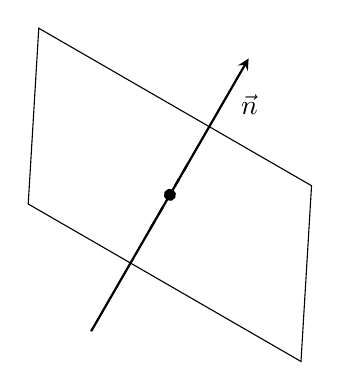
\begin{tikzpicture}
        % Rotate the entire picture 30 degrees clockwise
        \begin{scope}[rotate=-30]
          % Define coordinates for the parallelogram
          \coordinate (A) at (-2,-1);
          \coordinate (B) at (2,-1);
          \coordinate (C) at (1,1);
          \coordinate (D) at (-3,1);
          
          % Draw the parallelogram
          \draw (A) -- (B) -- (C) -- (D) -- cycle;
          
          % Draw the normal vector line
          \draw[-stealth, thick] (-0.5,-2) -- (-0.5,2);
          
          % Draw the dashed portion where the line intersects the parallelogram
          \draw[dashed, thick] (-0.5,-0.5) -- (-0.5,0.5);
          
          % Add a dot at intersection point
          \filldraw (-0.5,0) circle (2pt);
          
          % Label the normal vector
          \node at (-0.2,1.5) {$\vec{n}$};
        \end{scope}
      \end{tikzpicture}
      \caption{The linear operator that rotates around a vector $v$ by an angle $\theta$ has an eigendecomposition of the span of $v$ as shown (with eigenvalue $1$) and the 2-dimensional plane (having two complex eigenvalues). } 
      \label{fig:rotation}
    \end{figure}
	\end{example}

	\begin{example}[2 Rotations in $\mathbb{R}^4$]
		Observe the following JNF, with columns (from left to right) corresponding to the transformations $h_1$ (genuine), $k_1$ (generalized), $h_2$ (genuine), and $k_2$ generalized). 
		\begin{equation}
			\begin{pmatrix}
				e^{i \theta} & 1 & & \\
				& e^{i \theta} & & \\
				& & e^{-i \theta} & 1 \\
				& & & e^{i- \theta}
			\end{pmatrix}
		\end{equation}

		Using the corollary shown above, we can modify the eigenvalues and eigenvectors into real values and construct the simplest "real form" (assuming $i \neq 0, \pi$) of the matrix 
		\begin{equation}
			\begin{pmatrix}
				\cos{\theta} & - \sin{\theta} & 1 & 0 \\
				\sin{\theta} & \cos{\theta} & 0 & 1 \\
				0 & 0 & \cos{\theta} & - \sin{\theta} \\
				0 & 0 & \sin{\theta} & \cos{\theta}
			\end{pmatrix}
		\end{equation}

		where the columns (from left left to right) now correspond to transformation of real eigenvectors
		\begin{equation}
			\frac{h_1 + h_2}{2}, \frac{i(h_1 - h_2)}{2}, \frac{k_1 + k_2}{2}, \frac{i(k_1 - k_2)}{2}
		\end{equation}
		Therefore, we can state that the linear transformation represented by the two matrices in their respective bases are equivalent. 
	\end{example}

	\begin{theorem}[Similarity Conditions]
		$A, B \in \mathbb{R}^{n \times n}$ are similar if and only if their JNFs are the same. 
  \end{theorem}
  \begin{proof}
		We prove bidirectionally. 
		\begin{enumerate}
		  \item $(\rightarrow)$ $A \sim B \implies A = S^{-1} B S = S^{-1} P^{-1} J P S = (PS)^{-1} J (PS) \implies$ JNF of $A$ and $B$ are the same. 
			\item $(\leftarrow)$ $A$ and $B$ have same JNF $\implies A = P^{-1} J P, B = Q^{-1} J Q \implies J = Q B Q^{-1} \implies A = P^{-1} Q B Q^{-1} P = (Q^{-1} P)^{-1} B (Q^{-1} P) \implies A \sim B$. 
		\end{enumerate}
  \end{proof}

	\begin{theorem}[Diagonalizability Conditions for Multiplicities]
		A matrix $A \in \mathbb{R}^{n \times n}$ is diagonalizable if and only if its algebraic multiplicities is equal to its geometric multiplicities for all eigenvalues. 
  \end{theorem}
	\begin{proof}
	  We prove bidirectionally. 
		\begin{enumerate}
		  \item $(\rightarrow)$. If $A$ is diagonalizable, then the JNF will be diagonal, which implies that the algebraic multiplicities are equal to the geometric multiplicities. 
			\item $(\leftarrow)$. If the algebraic multiplicities are equal to the geometric multiplities, then the JNF will be diagonal and so $A$ is diagonalizable. 
		\end{enumerate}
	\end{proof}

	\begin{corollary}[Transposes are Similar]
		Let $A \in \mathbb{R}^{n \times n}$. Then, $A \sim A^T$. 
  \end{corollary}
  \begin{proof}
		It is sufficient to prove that $A$ and $A^T$ have the same eigendecomposition. Since $(A - \lambda I)^T = A^T - \lambda I$, $\det{(A - \lambda I)} = 0 \iff \det{(A - \lambda I)^T} = \det{(A^T - \lambda I)} \implies $ $A$ and $A^T$ have the same eigenvalues. Similarly, $\big( (A - \lambda I)^d \big)^T = (A^T - \lambda I)^d \implies$ the eigenspaces of $A$ and $A^T$ have the same dimension. 
  \end{proof}

\subsection{Spectral Mapping Theorem}

  \begin{theorem}[Spectral Mapping Theorem]
    Let $q$ be any polynomial, $A$ a square matrix with an eigenvalue $a$. Then: 
    \begin{enumerate}
      \item $q(a)$ is an eigenvalue of $q(A)$. 
      \item Every eigenvalue $q(A)$ is of the form $q(a)$, where $a$ is an eigenvalue of $A$. 
    \end{enumerate}
  \end{theorem}
  \begin{proof} 
    Listed. 
    \begin{enumerate}
      \item Let $h$ be an eigenvector of A with corresponding eigenvalue $a$. 
				\begin{align*}
					Ah = ah & \implies A^{2} h = Aah = aAh = a^{2} h \\
					 & \implies A^{n} h = a^{n} h   \\
					 & \implies q(A)h = q(a)h \\
					 & \implies q(a) \text{ is an eigenvalue of }q(A)
				\end{align*}

      \item Let $p$ be the eigenvalue of $q(A) \iff \det{\big(q(A) - p I\big)} = 0$. We expand: 
        \begin{equation}
          q(s) - p = c\prod \big(s-r_{i}\big), r_{i} \in \mathbb{C}
        \end{equation}
        Replacing the variable $s$ with $A$, we have
        \begin{equation}
          q(A) - pI = c \prod \big(A-r_{i}I\big)
        \end{equation}
        Since $\det{\big( q(A) - pI\big)} = 0$, at least one $r_{i}$, say $r_{k}$ exists such that $\det{\big( A - r_{k} I \big)} = 0 \iff r_{k}$ is an eigenvalue of $A$. Since $q(r_{j})-p = 0$, $p = q(r_{j})$ is an eigenvalue of $q(A)$. 
    \end{enumerate}
  \end{proof}

	Therefore if $A \in \mathbb{R}^{n \times n}$, $f$ is a polynomial, and if the chracteristic polynomial of $A$ has factorization 
	\begin{equation}
		p_A (t) = \prod_{i = 1}^n (t - \lambda_i)
	\end{equation}
	then the characteristic polynomial of the matrix $f(A)$ is given by 
	\begin{equation}
		p_{f(a)} (t) = \prod_{i = 1}^n (t - f(\lambda_i))
	\end{equation}

  \begin{theorem}[Cayley Hamilton]
    Every matrix $A$ satisfies its own characteristic equation. That is, 
		\begin{equation}
    	p_{A}(A) = 0
		\end{equation}
  \end{theorem} 
	\begin{proof}
	  
	\end{proof}

\subsection{Eigenvalue Bounds (Gershgorin)}

  We can actually create a bound on the spectrum of a square matrix. 

  \begin{theorem}[Gershgorin Circle Theorem]
		Let $A \in \mathbb{C}^{n \times n}$, and let us define the \textbf{Gershgorin disk} in the equivalent ways: 
		\begin{enumerate}
		  \item Let $R_i$ be the sum of the absolute values of the non-diagonal entries of the $i$th row, and let $D_(a_{i i}, R_i) \subset \mathbb{C}$ be a closed disk with radius $R_i$ centered at $a_{i i}$. 
		  \item Let $C_i$ be the sum of the absolute values of the non-diagonal entries of the $i$th column, and let $D_(a_{i i}, C_i) \subset \mathbb{C}$ be a closed disk with radius $C_i$ centered at $a_{i i}$. 
		\end{enumerate}

		Then, every eigenvalue of $A$ lies within the union of all $n$ Gershgorin Disks. That is, 
		\begin{equation}
    	\lambda_j (A) \in \bigcup_{i= 1}^{n} D_(a_{i i}, R_i) \subset \mathbb{C}, \text{ for all } j
		\end{equation}
  \end{theorem}
  \begin{proof}
    Let $\lambda$ be an eigenvalue of $A$ with its eigenvector $v = (v_j)$. Scale $v$ by multiplying it by $ \pm 1 / \max{\{|v_j|\}_j}$ to get a vector $x$ with its maximal entry $x_i = 1$ and $|x_j| \leq 1, \; j \neq i$. Then, 
		\begin{equation}
    	A x = \lambda x \implies \sum_{j} a_{i j} x_j = \lambda x_i = \lambda \implies \sum_{j \neq i} a_{i j} x_j + a_{i i} = \lambda
		\end{equation}
    Applying the triangle inequality, 
		\begin{equation}
    	| \lambda - a_{i i} | = \bigg| \sum_{j \neq i} a_{i j} x_j\bigg| \leq \sum_{j \neq i} |a_{i j}| |x_j| \leq \sum_{j \neq i} |a_{i j}| = R_i
		\end{equation}
    For the columns, this is a direct result from the fact that $A$ is similar to $A^T$. Alternatively, we can apply the same process in the proof above to $A^T$.
  \end{proof}

  If one observes that the off-diagonal entries of $A$ are small in absolute value, it can be concluded that the diagonal entries are "close" to the true eigenvalues of $A$. $A$ is diagonal if and only if the Gershgorin disks are points. 

\subsection{Self-Adjoint Operators}

  \begin{theorem}[Spectral Theorem]
    A $n$-dimensional self-adjoint map $H$ over $\mathbb{C}$ has real eigenvalues and an orthonormal basis of genuine eigenvectors. That is, its eigendecomposition consists of $n$ pairwise orthogonal eigenspaces. 
  \end{theorem}
	\begin{proof}
	  
	\end{proof}

  \begin{corollary}
    Given a real self-adjoint matrix $H$, there exists a real invertible matrix $M$ such that $M^\dagger H M = D$, with $D$ diagonal and the column vectors form an orthonormal basis.
  \end{corollary}
	\begin{proof}
	  
	\end{proof}

	So, given self-adjoint $H: X \longrightarrow X$, the whole space can be written as the direct sum of pairwise orthogonal eigenspaces. 
	\begin{equation}
		X = \bigoplus_{i=1}^n E(\lambda_i)
	\end{equation}

	\begin{definition}[Spectral Resolution]
    Given that $P_j$ is the orthogonal projection onto the $j$th eigenspace $E(\lambda_j)$, that is
    \begin{equation}
      P_j (x) = x_j \in E(\lambda_j), \; \text{ ($P_j$ also self adjoint)}
    \end{equation}
    the \textbf{spectral resolution} of self-adjoint mapping $H$ is the decomposition into the form 
    \begin{equation}
      H = \sum_j \lambda_j P_j \implies H x = \bigg( \sum_j \lambda_j P_j \bigg) x = \sum_j \lambda_j x_j
    \end{equation}
    The resolution of the identity is
    \begin{equation}
      I = \sum_j P_j
    \end{equation}
  \end{definition}

  \begin{theorem}
    Given the spectral resolution of self-adjoint $H$, 
    \begin{equation}
      H  = \sum_j \lambda_j P_j \implies H^2 = \sum_j \lambda_j^2 P_j
    \end{equation}
  \end{theorem}
	\begin{proof}
	  
	\end{proof}

  Note that the spectral resolution of a self adjoint mapping is precisely the eigendecomposition of the mapping into its 1-dimensional eigenspaces. It is merely a simpler form of the eigendecomposition in the specific case when the linear mapping is self-adjoint. 

	\begin{theorem}[Spectral Resolution of Commuting Self-Adjoint Operators]
    Let $H, K$ be self-adjoint mappings such that $H K = K H$. Then $H$ and $K$ have the same spectral resolution, i.e. they have the same eigendecomposition. 
    \begin{equation}
      H = \sum_j a_j P_j, \; \; K = \sum_j b_j P_j
    \end{equation}
  \end{theorem}
  \begin{proof}
    $x \in E(a) H x = a x \implies K H x = a K x \implies H K x = a K x \implies K x \in E(a)$. Similarly, we can do this with $K$ to find $x \in E(a) \implies H x \in E(a)$, meaning that $K$ and $H$ have the same eigendecompositions (though their eigenvalues are not necessarily equal). 
  \end{proof}

	So, given an anti-self adjoint map $A$, we can apply the spectral resolution to $iA$. 

	\begin{theorem}[Spectral Resolution of Anti-Self-Adjoint Operators]
    Given anti-self adjoint $A: \mathbb{C}^n \longrightarrow \mathbb{C}^n$, 
    \begin{enumerate}
      \item eigenvalues of $A$ are purely imaginary
      \item we can choose an orthonormal basis of eigenvectors of $A$
    \end{enumerate}
  \end{theorem}
  \begin{proof}
    This easily follows from the Spectral Theorem. 
  \end{proof}

  \begin{definition}[Normal Maps]
    $N: X \longrightarrow X$ is a \textbf{normal mapping} if $N^\dagger N = N N^\dagger$. 
  \end{definition}

	Self-adjoint, anti-self adjoint, and unitary matrices are all normal. Surprisingly, the set of normal matrices are not closed under addition nor multiplication, so they do not form a group. 

	\begin{theorem}[]
    A map $N$ is normal if and only if it has an orthonormal basis of eigenvectors, i.e. it is unitarily diagonalizable. That is, 
    \begin{equation}
      N = U^\dagger D U 
    \end{equation}
  \end{theorem}
  \begin{proof}
		We prove bidirectionally. 
		\begin{enumerate}
		  \item $(\rightarrow)$ Let 
				\begin{equation}
					H = \frac{1}{2} (N + N^\dagger), \; A = \frac{1}{2} (N - N^\dagger)
				\end{equation}
				$N^\dagger N = N N^\dagger \implies A H = H A$, where $H$ is self adjoint, $A$ is anti-self adjoint, and $N = H + A, N^\dagger = H - A$. Since $A H = H A$, they have the same spectral resolution of orthonormal eigenspaces, which also forms the same spectral resolution for $N = H + A$. \\

			\item $(\leftarrow)$ $A = U^\dagger D U \implies A^\dagger A = (U^\dagger D U) (U^\dagger \bar{D} U) = U^\dagger D \bar{D} U = A A^\dagger$. 
		\end{enumerate}
  \end{proof}

\subsection{Positive Definite Maps}

  \begin{definition}[Spectral Radius]
    The \textbf{spectral radius} of $A$ is defined
    \begin{equation}
      r(A) \equiv \max_i |a_i|, \; a_i \text{ are eigenvalues}
    \end{equation}
  \end{definition}

  \begin{definition}[Positive-Semidefinite]
    A self-adjoint linear mapping $H$ from a real or complex Euclidean space onto itself is \textbf{positive definite} if 
    \begin{equation}
      (x, H x) > 0 \text{ for all } x \neq 0
    \end{equation}
    $H$ is called \textbf{positive semidefinite} if 
    \begin{equation}
      (x, H x) \geq 0
    \end{equation}
  \end{definition}

  \begin{theorem}[Properties of Positive Definite Matrices] 
    Here we state basic properties. 
    \begin{enumerate}
      \item $I$ is positive definite. 
      \item Positive mappings form a subspace in the space of linear mappings. 
      \begin{align*}
        &M, N \text{ positive} \implies M + N \text{ is positive} \\
        &M \text{ positive} \implies a M \text{ is positive for all} a \in \mathbb{F}
      \end{align*}
      \item $H$ positive and $Q$ invertible $\implies Q^\dagger H Q$ positive. 
    \end{enumerate}
  \end{theorem}

  \begin{theorem}
    $H$ is positive definite if and only if all of its eigenvalues are positive. Furthermore, every positive mapping is invertible.
  \end{theorem}

  \begin{theorem}
    Every positive mapping $M$ has a unique positive square root. That is, there exists a unique positive mapping $N$ such that
    \begin{equation}
      N^2 = M 
    \end{equation}
    We denote $N$ as $\sqrt{M}$. 
  \end{theorem}

  \begin{definition}
    Given that $M, N$ are positive definite mappings. 
    \begin{equation}
      M > N \iff M - N > 0, \text{ that is, $M$ is positive}
    \end{equation}
  \end{definition}

  \begin{theorem}
    If $M, N$ are positive definite mappings 
    \begin{equation}
       M > N \implies M^{-1} < N^{-1}
    \end{equation}
  \end{theorem}

  \begin{theorem}
    In $\mathbb{R}^n$ endowed with the dot product, a $n \times n$ matrix $A$ is positive definite if and only if 
    \begin{equation}
      (x, A y) = x^T A y > 0 
    \end{equation}
    for every $x, y \in \mathbb{R}^n$. $A$ is positive semi-definite if and only if 
    \begin{equation}
      (x, A y) = x^T A y \geq 0
    \end{equation}
  \end{theorem}

  The following is a useful fact regarding inner products of $\mathbb{R}^n$. 

  \begin{theorem}
    The set of all inner products that can be defined on $\mathbb{R}^n$ is bijective to the set of positive-definite symmetric $n \times n$ matrices $A$ (which is itself bijective to the set of all positive-definite mappings). That is, every inner product of $\mathbb{R}^n$ can be defined 
    \begin{equation}
      (x, y) \equiv x^T A y
    \end{equation}
    Note that when $A = I_n$, the inner product is the regular dot product.
  \end{theorem}

\subsection{Singular Value Decomposition} 

  We now proceed to another crucial decomposition, called the singular value decomposition. While the JNF allows us to choose the most convenient choice of basis for a square matrix, the Singular Value Decomposition (SVD) allows us to decompose general $m \times n$ matrices. 

  \begin{theorem}[Singular Value Decomposition]
    Any linear mapping $M$ from an $n$-dimensional inner product space to a $m$-dimensional inner product space can be decomposed into 
    \begin{equation}
      M = U \Sigma V^\dagger = \begin{pmatrix}
       \vert & \vert & \vert & \vert\\
      y_1 & y_2 & \ldots & y_m \\
      \vert & \vert & \vert & \vert
      \end{pmatrix}\begin{pmatrix}
      \sigma_1 & & & &0\\
      &\ddots &&& \vdots \\
      & & \sigma_p & & 0\\
      & & & \ddots &\vdots \\
      0 & \ldots &0& \ldots &0
      \end{pmatrix} \begin{pmatrix}
      \text{---}&x_1&\text{---} \\
      \text{---}&x_2&\text{---} \\
      \text{---}&\vdots&\text{---} \\
      \text{---}&x_n&\text{---}
      \end{pmatrix}
    \end{equation}
    where $U \in U(m), V \in U(n)$ and $\Sigma$ has diagonal elements with nonnegative real entries. Also, $p = $ rank$(M) \leq \min{\{n,m\}}$. This form is known as the \textbf{singular value decomposition}. The columns of $U$, denoted $y_i$, are called the \textbf{left singular vectors} and the columns of $V$ (i.e. the rows of $V^\dagger$), denoted $x_i$, are called the \textbf{right singular vectors}. The diagonal entries of $\Sigma$ are called the \textbf{singular values}. The SVD is unique up to the order of singular values, but it is generally constructed so that $\sigma_1 \geq \sigma_2 \geq \ldots \geq \sigma_p$. 
  \end{theorem}

  To provide a brief, yet unrigorous, justificiation of why the SVD exists, we look at the linear mapping $M: X \longrightarrow Y$, with $\dim{X} = n, \dim{Y} = m$. If $M$ is injective $(\iff m \geq n)$, given the basis $\{e_i\}$ for $X$, we can complete the linearly independent set $\{Me_i\}_{i=1}^n$ to a basis in $Y$ and represent $M$ as the mapping
  \begin{equation}
    \Sigma_{inj} = \begin{pmatrix} &&\\ &I_n&\\ &&\\ 0&\ldots &0 \end{pmatrix}
  \end{equation}
  If $M$ is surjective $(\iff m \leq n)$, then given basis $\{f_i\}_{i=1}^m$ of $Y$, we can choose a basis $\{e_j\}_{j=1}^n$ of $X$ such that $M(e_i) = f_i (i = 1, 2, \ldots, m)$, and $M(e_i) = 0$ when $i > m$. This produces the matrix
  \begin{equation}
    \Sigma_{surj} = \begin{pmatrix} &&&0\\&I_m&& \vdots \\&&&0\end{pmatrix}
  \end{equation}
  We now present the following theorem without proof. 

  \begin{theorem}
    Any map $M: X \longrightarrow Y$ can be written as a surjective map followed by an injective map. 
  \end{theorem}

  This theorem implies that any map, when given the right choice of basis, can be written as 
  \begin{equation}
    \Sigma_{inj} \Sigma_{surj} = \begin{pmatrix}
    &&&\cdots&0\\
    &I_p&&\cdots&0\\
    &&&\cdots&\cdots\\
    \cdots&\cdots&\cdots&\cdots&0\\
    0&0&\cdots&0&0
    \end{pmatrix} = \begin{pmatrix}
    1&&&&0\\
    &\cdots&&&\cdots\\
    &&1&&0\\
    &&&\cdots&\cdots\\
    0&\cdots&0&\cdots&0
    \end{pmatrix}
  \end{equation}
  where rk$(M) = p = $ the number of $1$'s in $\Sigma_{inj} \Sigma_{surj}$. As for choosing the proper set basis for $X$ and $Y$, we can find these passive transformations in the unitary groups $U(n)$ and $U(m)$. 

  We now present a geometric description of the singular value decomposition. Think of the unit $n$-ball being rotated and flipped ($V^\dagger$ applied) under the unitary transformation. Then, it is stretched along its othogonal axes to result in an ellipsoid living in an $m$-dimensional space. The factor of stretching and compressing the axes are precisely the singular values. Finally, this ellipsoid is rotated and flipped ($U$ applied) back to its original basis. 

  \begin{theorem}
    Geometrically, we can see that the largest singular value is the matrix norm, also called the operator norm. 
    \begin{equation}
      \|M\| = \sigma_1
    \end{equation}
  \end{theorem}

  \begin{theorem}[Properties of Singular Values] 
    Given linear mapping $A$ from a $n$-dimensional inner product space to $m$-dimensional inner product space, 
    \begin{enumerate}
      \item $\sigma_i(A) = \sigma_i (A^T) = \sigma_i (A^\dagger) = \sigma_i (\bar{A})$

      \item $\forall \; U \in U(m), V \in U(n), \; \sigma_i (A) = \sigma_i (U A V)$

      \item Relation to eigenvalues
      \begin{equation}
        \sigma_i^2(A) = \lambda_i (A^\dagger A) = \lambda_i (A A^\dagger)
      \end{equation}
    \end{enumerate}
  \end{theorem}

  We now present the (not the best) process of computing SVD of small matrices by hand. Given matrix $M$, $M = U \Sigma V^\dagger \implies M^\dagger M = V \Sigma^2 V^\dagger$. The eigenvalues of $M^\dagger M$ are $\sigma_i^2$ with corresponding eigenvectors being the columns of $V$, which can all be found by putting $M^\dagger M$ into JNF. We repeat this process for $M M^\dagger = U \Sigma^2 U^\dagger$ to find the eigenvectors that make up the column vectors of $U$. 

  \begin{theorem}
    Let $A: X \longrightarrow Y$, with $\dim{X} = n, \dim{Y} = m$, and let $k \leq \min{\{m, n\}}$, with $A = U \Sigma V^\dagger$. Then, amongst all rank $k$ $m \times n$ matrices $B$, the matrix $A^{(k)}$ minimizes 
    \begin{equation}
      \|A-B\|_2, \; A^{(k)} = U \Sigma^{(k)} V^\dagger
    \end{equation}
    and $\Sigma^{(k)}$ is $\Sigma$ with $\sigma_{k+1} = \sigma_{k+2} = \cdots = 0$. Therefore, to see how "close" $B$ is to $A$, we can compare the singular values of $A$ and $B$, given that they both have the same unitary matrices $U$ and $V$. 
  \end{theorem}

  The singular value decomposition has many applications in high dimensional data analysis and data compression. For example, in a set of $m$ data points in $\mathbb{R}^n$ that each lie in the rows of matrix $A$, if the singular values of $A$ suddenly drops (e.g. $120, 118, 107, 98, 2, 1, 0.3, \cdots$) then we can determine that the points "almost" lie in a subspace in $\mathbb{R}^n$. Knowing this allows us to compress high dimensional data to $A^{(k)}$, which is a more manageable form. This is especially useful in the data compression of electronic images, where each pixel is treated as a single number to form a matrix. 

  It can also be used to define the "pseudo-inverse" of a matrix that may not be invertible. 

  \begin{definition}[Pseudo-Inverse]
    Given matrix $M = U \Sigma V^\dagger$ in SVD, we define the \textbf{pseudo-inverse} $M^+ = V \Sigma^+ U^\dagger$, where $\Sigma^+$ is $\Sigma$ with entries $\sigma_i^{-1}$, or $0$ if $\sigma_i = 0$. For example,
    \begin{equation}
      \Sigma = \begin{pmatrix}3&0&0\\0&2&0\\0&0&0\end{pmatrix} \implies \Sigma^+ = \begin{pmatrix}1/3&0&0\\0&1/2&0\\0&0&0\end{pmatrix}
    \end{equation}
    $\implies M^+ M = V \Sigma^+ \Sigma V^\dagger$. If $M$ is square and all $\sigma_i \neq 0$, then $M^\dagger M = V V^\dagger \implies M^\dagger M = I \implies  M^+ = M^{-1}$. 
  \end{definition}

  By computing the SVD of $M$, where $\sigma_p \neq 0, p =$ rk$\,M = $ rk$\,\Sigma$, we can automatically compute the 4 fundamental spaces. 
  \begin{equation}
    M = U \Sigma V^\dagger = \begin{pmatrix}&&&&|&\\&&&&|&\\&&U&&|&U^\prime\\&&&&|&\\&&&&|&
    \end{pmatrix} \begin{pmatrix}
    \sigma_1&&&&0\\
    &\sigma_2&&&0\\
    &&\cdots&&\cdots\\
    &&&\sigma_p&0\\
    0&0&\cdots&0&0
    \end{pmatrix}\begin{pmatrix}
    &&&&\\&&&&\\&&V^\dagger&&\\&&&&\\\text{---}&\text{---}&\text{---}&\text{---}&\text{---}
    \\&&V^{\dagger \prime}&&
    \end{pmatrix}
  \end{equation}
  \begin{enumerate}
    \item $\im{M} = C(U)$
    \item $\ker{M} = R(V^{\dagger \prime}) = C(V^\prime)$
    \item $\ker{M^\dagger} = C(U^\prime)$
    \item $\im{M^\dagger} = C(V) = R(V^\dagger)$
  \end{enumerate}

  One of the main differences between the JNF and SVD of a matrix $A$ lies in how they are affected by perturbations in the elements of $A$. For example, take the small change 
  \begin{equation}
    A = \begin{pmatrix}
    1 & 1\\
    0 & 1
    \end{pmatrix} \longrightarrow A^\prime  = \begin{pmatrix}
    1 & 1 \\
    0 & 1.00001
    \end{pmatrix}
  \end{equation}
  The SVD of $A^\prime$ will "change" continuously for changes in the elements of $A$, but the JNF of $A$ is completely different from the JNF of $A^\prime$. More specifically, the JNF of $A$ is $A$ itself, but the JNF os $A^\prime$ is now diagonalizable, meaning that the 2-dimensional eigenspace $E(1)$ "breaks up" into two 1-dimensional eigenspaces from small perturbations. 

  \begin{definition}[Frobenius Norm]
    The \textbf{Frobenius norm} of a $m \times n$ matrix $A$ is defined
    \begin{equation}
      \|A\|_F \equiv \sqrt{\Tr{(A^\dagger A)}} = \sqrt{\Tr{\Sigma^2}} = \bigg( \sum_{i, j} a_{i j}^2 \bigg)^{\frac{1}{2}} 
    \end{equation}
    By Singular Value Decomposition, we can reduce its calculations to
    \begin{equation}
      \|A\|_F = \sqrt{\sum_i \sigma_i^2}
    \end{equation}
    where $\sigma_i$'s are the singular values. Clearly, 
    \begin{equation}
      \|A\|_2 \leq \|M\|_F
    \end{equation}
    In quantum mechanics, the Frobenius norm is also called the \textbf{Hilbert Schmidt norm} in the context of infinite dimensional Hilbert spaces. 
  \end{definition}

  We end by defining two more common decompositions of square matrices. 

  \begin{theorem}[Schur Decomposition]
    Every $n \times n$ matrix $A$ over $\mathbb{C}$ can be decomposed into
    \begin{equation}
      A = Q T Q^\dagger
    \end{equation}
    where $Q \in U(n)$ and $T$ is upper triangular. 
  \end{theorem}
  \begin{proof}
    This is an obvious result of the Grahm-Schmidt algorithm. 
  \end{proof}

  \begin{theorem}[Polar Decomposition]
    Every complex $n \times n$ matrix $A$ can be factored into the form
    \begin{equation}
      A = U P
    \end{equation}
    where $U \in U(n)$ and $P$ is a positive semidefinite self-adjoint matrix. If $A$ is a real matrix, then $U \in O(n)$. 
  \end{theorem}
  \begin{proof}
    We take the SVD to get 
    \begin{equation}
      A = W \Sigma V^\dagger
    \end{equation}
    and we can assign 
    \begin{equation}
      U = W V^\dagger, \; P = V \Sigma V^\dagger
    \end{equation}
    Since $V, W$ are unitary, this confirms that $P$ is positive definite and self-adjoint along with $U$ being unitary. Thus, the existence of the SVD implies the existence of the polar decomposition. 
  \end{proof}

\subsection{Polar Decomposition}

  \begin{theorem}[Polar Decomposition]
    Given a Euclidean space $\mathbb{E}^n$ and any linear endomorphism $f$ of $\mathbb{E}^n$, there are two positive definite self-adjoint linear maps $h_1, h_2 \in$ End$(\mathbb{E}^n)$ and $g \in$ O$(n)$ such that
    \begin{equation}
      f = g \circ h_1 = h_2 \circ g
    \end{equation}
    That is, such that $f$ can be decomposed into the following as shown in this commutative diagram. 
    \begin{tikzcd}
      \mathbb{E}^n \arrow{r}{h_2} & \mathbb{E}^n \\
      \mathbb{E}^n \arrow{u}{g} \arrow{ur}{f} \arrow{r}{h_1} & \mathbb{E}^n \arrow{u}{g}
    \end{tikzcd}
  \end{theorem}

